\subsubsection{UML Description}
The UML below describes at high-level the model of the system to be developed. It considers the basic service together with the advanced function 1 and advanced function 2 previously specified. The UML does not include every class that will be necessary to define the complete architecture of the system.\\
CLup has more functions than basic service. The manager registers to the application with all necessary information and the manager could activate the advance function 1 or advance function 2 at any time. The user who use mobile could simply download the application on his/her device and use it and user who doesn't have mobile could easily go near the shop and get a ticket from ticket machine.\\
Here we can identify the main aspect of CLup:
\begin{itemize}
    \item The user could request to be in line for a shop and application shows estimated waiting time to him/her.
    \item The user could book a visit for a shop. This booking contains the date and time user wants to go shopping. Besides, user can add the categories of item he/she has in shopping list. The application could suggest the user free slots and user book them.
    \item The application based the current location of users must notify them and ask them to approach the shop in a suitable time.
    \item The application must notify people when it's their turn to go shopping.
    \item At the entrance time, the QR code generated in the app must be scanned to ensure they come in the right time.
    \item At the checkout, the clerk must scan the QR code of user and the system must add shopping information (like duration of shopping, category of item which user buy) to user history.
\end{itemize}

\begin{figure}[H]
  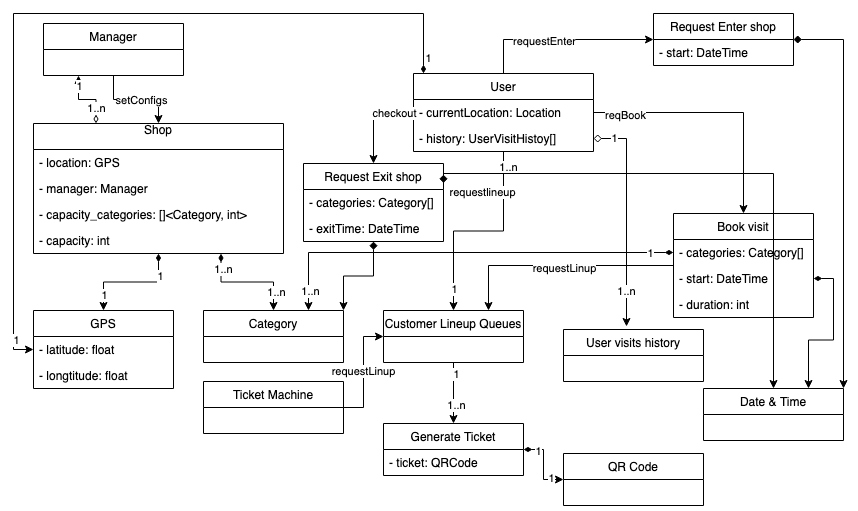
\includegraphics[width=\textwidth,height=\textheight,keepaspectratio]{images/ClassDiagram.png}
  \caption{High level Class Diagram}
  \label{fig:ClassDiagram}
\end{figure}

\subsubsection{State Diagrams}
Now we analyse the some important functions of the application, modelling their behaviours and analyze their behaviour to have the expected functionality. we report these diagrams below. \\

\begin{figure}[H]
  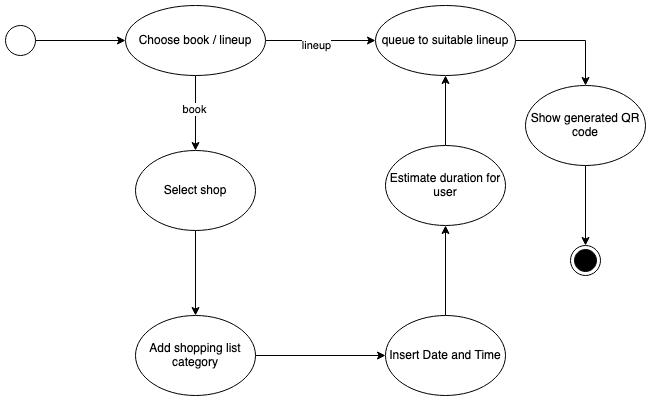
\includegraphics[width=\textwidth,height=\textheight,keepaspectratio]{images/bookLineup.png}
  \caption{User book a visit or insert to lineup queue}
  \label{fig:bookLineup}
\end{figure}

In this (Figure \ref{fig:bookLineup}), we model a user whom has a cell phone and wants to go shopping. As you can see, the user can choose to go to queue or book a visit for a time in future.

\begin{figure}[H]
  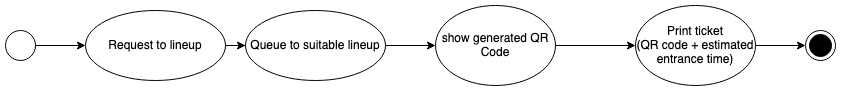
\includegraphics[width=\textwidth,height=\textheight,keepaspectratio]{images/OfflineTicket.png}
  \caption{User get ticket from ticket machine}
  \label{fig:OfflineTicket}
\end{figure}

In this (Figure \ref{fig:OfflineTicket}), we model a user who want to use ticket machine and do not use the app. In this case, user only can add himself/herself to the current line up of the shop.

\begin{figure}[H]
  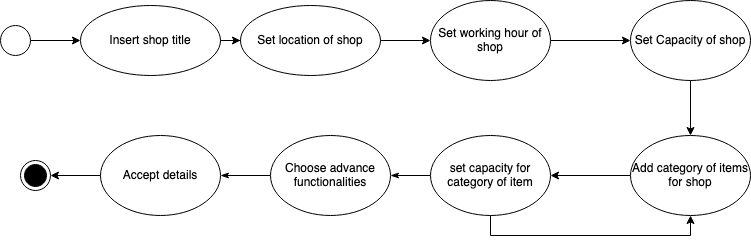
\includegraphics[width=\textwidth,height=\textheight,keepaspectratio]{images/CreateShop.png}
  \caption{Manager create a shop}
  \label{fig:CreateShop}
\end{figure}

In this (Figure \ref{fig:CreateShop}), shows how a manager could create a shop and add necessary information for creating a shop in our system.

\begin{figure}[H]
  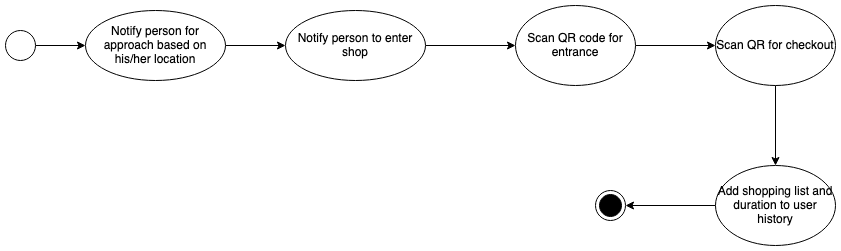
\includegraphics[width=\textwidth,height=\textheight,keepaspectratio]{images/Shopping.png}
  \caption{User shopping}
  \label{fig:shopping}
\end{figure}

In this (Figure \ref{fig:shopping}), we model the behaviour of user from entrance to shop until checkout. In the checkout time, we re-scan the QR code of user to insert data user shopping list and duration to user history. we could use, this information to estimate the behaviour of each user and improve waiting time estimation in our system.

\begin{figure}[H]
  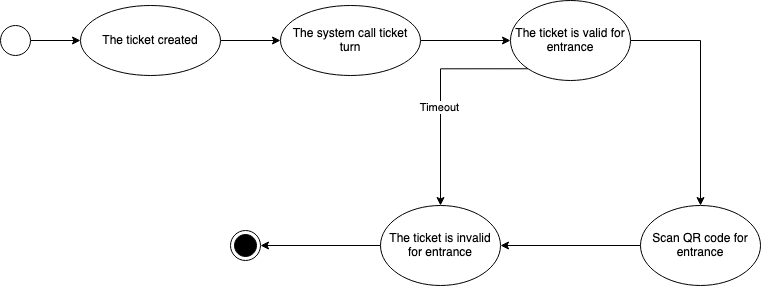
\includegraphics[width=\textwidth,height=\textheight,keepaspectratio]{images/Ticket.png}
  \caption{Ticket states}
  \label{fig:ticket}
\end{figure}

In this (Figure \ref{fig:ticket}), the life cycle of a ticket shows. This helps us to understand when a ticket is valid for enter the shop.